\documentclass{article}
\usepackage{amsmath, amsthm, amssymb, amsfonts}
\usepackage{thmtools}
\usepackage{graphicx}
\usepackage{setspace}
\usepackage{geometry}
\usepackage{float}
\usepackage{hyperref}
\usepackage[utf8]{inputenc}
\usepackage[english]{babel}
\usepackage{framed}
\usepackage[dvipsnames]{xcolor}
\usepackage{tcolorbox}

%% ggraoph 

\usepackage {tikz}
\usetikzlibrary {positioning}
\definecolor {processblue}{cmyk}{0.96,0,0,0}

\colorlet{LightGray}{White!90!Periwinkle}
\colorlet{LightOrange}{Orange!15}
\colorlet{LightGreen}{Green!15}

\newcommand{\HRule}[1]{\rule{\linewidth}{#1}}

\colorlet{LightGray}{black!10}
\colorlet{LightOrange}{orange!15}
\colorlet{LightGreen}{green!15}
\colorlet{LightBlue}{blue!15}
\colorlet{LightCyan}{cyan!15}



\declaretheoremstyle[name=Theorem,]{thmsty}
\declaretheorem[style=thmsty,numberwithin=section]{theorem}
\usepackage{tcolorbox} % Add missing package
\tcolorboxenvironment{theorem}{colback=LightGray}

\declaretheoremstyle[name=Definition,]{thmsty}
\declaretheorem[style=thmsty,numberwithin=section]{definition}
\tcolorboxenvironment{definition}{colback=LightBlue}

\declaretheoremstyle[name=Proposition,]{prosty}
\declaretheorem[style=prosty,numberlike=theorem]{proposition}
\tcolorboxenvironment{proposition}{colback=LightOrange}


\declaretheoremstyle[name=Proof,]{prosty}
\declaretheorem[style=prosty,numberlike=theorem]{proofbox}
\tcolorboxenvironment{proofbox}{colback=LightOrange}

\declaretheoremstyle[name=Axiom,]{prcpsty}
\declaretheorem[style=prcpsty,numberlike=theorem]{axiom}
\tcolorboxenvironment{axiom}{colback=LightGreen}

\declaretheoremstyle[name=Lemma,]{prcpsty}
\declaretheorem[style=prcpsty,numberlike=theorem]{lemma}
\tcolorboxenvironment{lemma}{colback=LightCyan}





\setstretch{1.2}
\geometry{
    textheight=9in,
    textwidth=5.5in,
    top=1in,
    headheight=12pt,
    headsep=25pt,
    footskip=30pt
}

% ------------------------------------------------------------------------------

\begin{document}

% ------------------------------------------------------------------------------
% Cover Page and ToC
% ------------------------------------------------------------------------------

\title{ \normalsize \textsc{}
		\\ [2.0cm]
		\HRule{1.5pt} \\
		\LARGE \textbf{\uppercase{Lecture 1 }}
		\HRule{2.0pt} \\ [0.6cm] \LARGE{}
		}

\date{\today}
\author{\textbf{Author} \\ 
		Tom Jeong
        }

\maketitle
\newpage

\tableofcontents
\newpage

% ------------------------------------------------------------------------------

\section{Graph Theory Basics}
A graph is a mathematical object consisting of: \begin{enumerate}
    \item vertices
    \item edges which is a pair of vertices
\end{enumerate}
Typically, we represent vertices as dots and edges as line segments that joins two dots. 
e.g. $G = (V, E)$ where $V$ is a set of vertices and $E$ is a set of edges. drawing a graph using tikz: 
\begin{center}
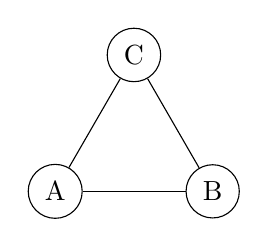
\begin{tikzpicture}
    \node[shape=circle,draw=black] (A) at (0,0) {A};
    \node[shape=circle,draw=black] (B) at (2,0) {B};
    \node[shape=circle,draw=black] (C) at (1,1.732) {C};
    \draw (A) -- (B);
    \draw (B) -- (C);
    \draw (C) -- (A);
\end{tikzpicture}
\end{center}

Given a graph $G$ we'll denote its vertex set by $V(G)$ and its edge set by $E(G)$.
\end{document}
